\subsection{Soluzione esercizio 8.2 Hoff}

Sensitivity analysis: In this exercise we will revisit the study from Exercise 5.2, in which 32 students in a science classroom were randomly assigned to one og two study methods, A and B, with $n_A = n_B = 16$. After several weeks of study, students were examined on the course material, and the scores are summarized by $\{\bar{y}_A = 75.2, s_A = 7.3\}, \{\bar{y}_B = 77.5, s_B = 8.1\}$. We will estimate $\theta_A = \mu+\delta$ and $\theta_B = \mu-\delta$ using the two-sample model and prior distributions of Section 8.1.
\begin{itemize}
	\item[a)] Let $\mu \sim $normal(75,100),  $1/\sigma^2\sim$ gamma(1,100) and $\delta\sim$normal$(\delta_0, \tau^2_0)$. For each combination of $\delta_0 \in \{-4, -2, 0, 2, 4\}$ and $\tau_0 \in \{10, 50, 100, 500\}$, obtain the posterior distribution of $\mu$, $\delta$ and $\sigma^2$ and compute
	\begin{itemize}
		\item[i.] Pr$(\delta>0|\boldsymbol{Y})$;
		\item[ii.] a 95$\%$ posterior confidence interval for $\delta$;
		\item[iii.] the prior and posterior correlation of $\theta_A$ and $\theta_B$.
	\end{itemize}
	\item[b)] Describe how you might use these results to convey evidence that $\theta_A<\theta_b$ to people of a variety of prior opinions.
\end{itemize}

\textbf{Svolgimento}
\bigskip

L'obiettivo di questo esercizio e'\ quello di condurre un'analisi di sensitivita\'. Ossia, si vuole valutare il cambiamento dell'inferenza al variare della specificazione della prior. Dato il modello delle osservazioni 
\[
Y_{iA} = \mu + \delta + \varepsilon_{iA};
\]
\[
Y_{iB} = \mu - \delta + \varepsilon_{iB} = \varepsilon_{iB};
\]
\[
\varepsilon_{ij} | \sigma^2 \sim i.i.d \quad N(0,\sigma^2) \quad j = A,B;
\]
\[
\mu|\gamma_0^2,\mu_0 \sim N(\mu_0,\gamma_0^2);
\]
\[
\mu|\tau_0^2,\delta_0 \sim N(\delta_0,\tau_0^2);
\]
\[
\sigma^2 | \nu_0,\sigma_0^2 \sim inverse-Gamma(\frac{\nu_0}{2},\frac{\nu_0\sigma^2}{2})
\]
\[
p(\mu,\delta,\sigma^2) = p(u)p(\delta)p(\sigma^2)
\]
e la sua rappresentazione tramite DAG in Figura \ref{figure:dag}
\begin{figure}
 \centering
 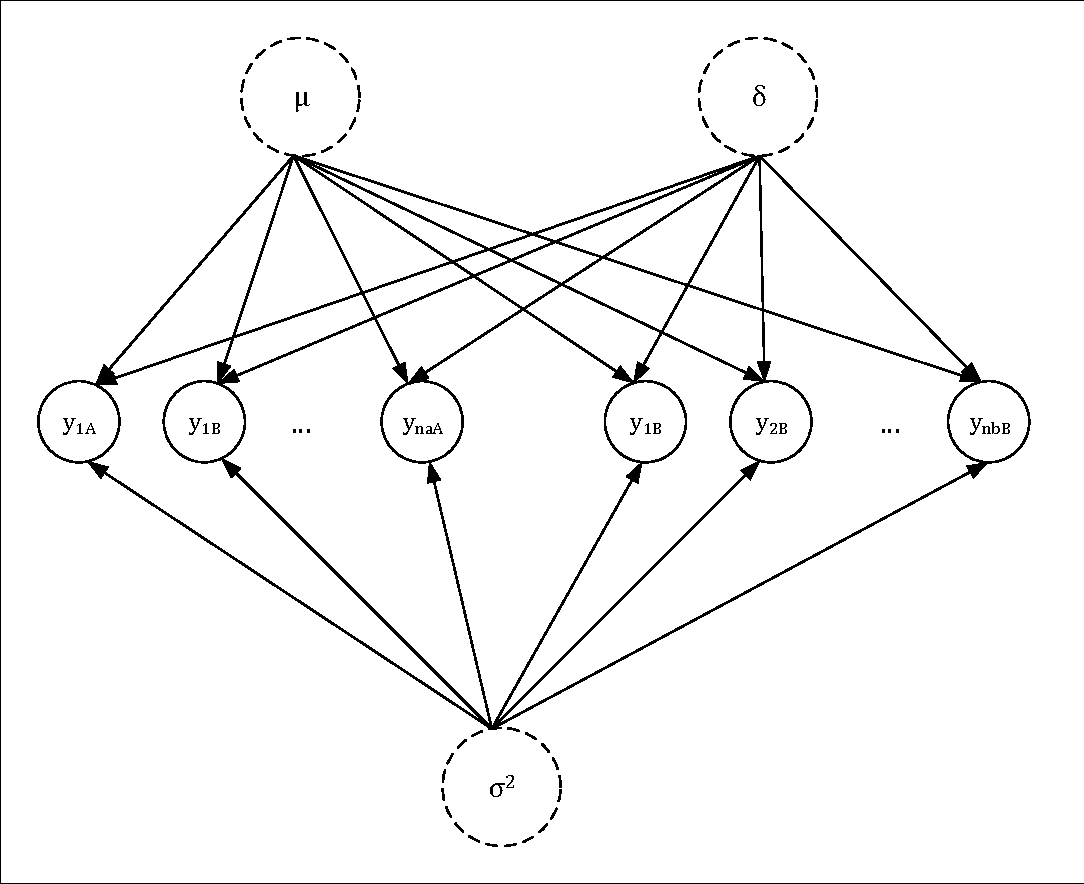
\includegraphics[scale=0.6]{img/DAG}
 
 \caption{DAG: confronto tra due popolazioni normali}
 \label{figure:dag}
\end{figure}
\begin{itemize}
\item Assegniamo agli iperparametri i valori che sono stati richiesti
\[
\mu_0 = 75; \quad \gamma_0^2 = 100; \quad \frac{\nu}{2} = 1 \implies \nu_0 = 2; \quad \frac{\nu_0\sigma_0^2}{2}=100
\]
\[
\implies \sigma_0^2 = 100;
\]
\[
\delta_0 \in \{-4,-2,0,2,4\}; \quad \tau_0^2 \in \{10,50,100,500\}
\]
avendo i seguenti dati campionari
\[
\bar{y_A} = 75.2, \quad s_A = 7.3, n_A = 16;
\]
\[
\bar{y_B} = 77.5, \quad s_B = 8.1, n_B = 16;
\]
\[
n_j=n=16; \quad \bar{y_j}=\frac{1}{n_j}\sum_{i=1}^{n_j}y_{ij}; \quad s_j = \sqrt{\frac{1}{n_j-1}\sum_{i=1}^{n_j}(y_{ij}-\bar{y_j})^2}
\]
per fare l'inferenza richiesta e'\ necessario determinare la distribuzione a posteriori delle variabili $\mu,\delta,\sigma^2$, ossia
$$p(\mu,\delta,\sigma^2|y_{1A},\dots,y_{n_AA},y_{1B},\dots,y_{n_BB}).$$ 
Per far cio'\ approssimiamo tale distribuzione mediante campionamento MCMC, secondo l'ottica Gibbs. Le distribuzioni full conditional dei parametri sono quindi le seguenti:
\[
\sigma^2 | y_{1A},\dots,y_{n_AA},y_{1B},\dots,y_{n_BB}, \mu, \delta \sim inverse-Gamma(\frac{\nu_n}{2},\frac{\nu_n\sigma_n^2}{2}) 
\]
in cui 
\[
\nu_n = \nu_0 + n_A + n_B;
\]
\[
\nu_n \sigma_n^2=\nu_0\sigma_0^2+\sum_{i=1}^{n_A}[y_{iA}-(\mu+\delta)]^2+ \sum_{k=1}^{n_B}[y_{kB}-(\mu-\delta)]^2=
\]
\[
=\nu_0\sigma_0^2 + \sum_{i=1}^{n_A}[y_{iA}^2-2(\mu+\delta)y_{iA} + (\mu + \delta)^2] +
\]
\[
 +\sum_{k=1}^{n_B}[y_{kB}^2-2(\mu-\delta) + (\mu - \delta)^2]=
\]
\[
=\nu_0\sigma_0^2 + \sum_{i=1}^{n_A}y_{iA}^2 - 2(\mu + \delta)\sum_{i=1}^{n_A}y_{iA} + n_A(\mu + \delta)^2+ 
\]
\[
+ \sum_{k=1}^{n_B}y_{kB}^2 - 2(\mu-\delta)\sum_{k=1}^{n_B}y_{kB} + n_B(\mu-\delta)^2=
\]
\[
\nu_0\sigma_0^2+(n_A-1)s_A^2+n_A\bar{y}_A^2-2(\mu + \delta)n_A\bar{y}_A+n_{A}(\mu+\delta)^2+
\]
\[
+(n_B-1)s_B^2+n_B\bar{y}_B^2-2(\mu-\delta)n_B\bar{y}_B+n_B(\mu-\delta)^2=
\]
\[
+n_B(\mu-\delta)^2=\nu_0\sigma_0^2 +(n-1)(s_A^2+s_B^2)+n(\bar{y}_A^2+\bar{y}_B^2)+
\]
\[
+n[-2(\mu+\delta)\bar{y}_A+(\mu+\delta)^2-2(\mu-\delta)\bar{y}_B+(\mu-\delta)^2=
\]
\[
\nu_0\sigma_0^2+(n-1)(s_A^2+s_B^2)+n(\bar{y}_A^2+\bar{y}_B^2)+
\]
\[
+2n[-\mu(\bar{y}_A+\bar{y}_B)+\delta(\bar{y}_B-\bar{y}_A)+\mu^2 + \delta^2].
\]
\[
\mu|y_{1A},\dots,y_{nA},y_{1B},\dots,y_{nB},\delta,\sigma^2 \sim N(\mu_n,\gamma_n^2)
\]
in cui 
\[
\gamma_n^2=[\frac{1}{\gamma_0^2}+\frac{(n_A+n_B)}{\sigma^2}]^{-1} = \frac{\gamma_0\sigma^2}{\sigma^2+(n_A+n_B)\sigma_0^2};
\]
\[
\mu_n =\gamma_n^2[\frac{\mu_0}{\gamma_0^2}+\frac{1}{\sigma^2}\sum_{i=1}^{n_A}(y_{iA}-\delta)+\frac{1}{\sigma^2}\sum_{k=1}^{n_B}(y_{kB}+\delta)]= 
\]
\[
=\gamma_n^2[\frac{\mu_0}{\gamma_0^2}+\frac{1}{\sigma^2}[(\sum_{i=1}^{n_A}y_{iA}) - n_A\delta + (\sum_{k=1}^{n_B}y_{kB} + n_B\delta)]]=
\]
\[
= \gamma_n^2[\frac{\mu_0}{\gamma_0^2}+\frac{1}{\gamma^2}(n_A\bar{y}_A-n_A\delta+n_B\bar{y}_B+n_B\delta)] = 
\]
\[
=\gamma_n^2[\frac{\mu_0}{\gamma_0^2}+\frac{n}{\sigma^2}(\bar{y}_A+\bar{y}_B)].
\]
\[
\delta | y_{1A},\dots,y_{n_aA},y_{1B},\dots,y_{n_BB},\mu,\delta^2 \sim N(\delta_n,\tau_n^2)
\]
in cui
\[
\tau_n^2 = (\frac{1}{\tau_0^2}+\frac{n_A+n_B}{\sigma^2})^{-1} = \frac{\sigma^2\tau_0^2}{\sigma^2+(n_A+n_B)\tau_0^2};
\]
\[
\delta_n = \tau_n^2[\frac{\delta_0}{\tau_0^2}+\frac{1}{\sigma^2}\sum_{i=1}^{n_A}(y_{iA}-\mu)-\frac{1}{\sigma^2}\sum_{k=1}^{n_B}(y_{kB}-\mu)]=
\]
\[
\tau_n^2[\frac{\delta_0}{\tau_0^2}+\frac{1}{\sigma^2}[(\sum_{i=1}^{n_A}y_{iA}-n_A\mu)+(\sum_{k=1}^{n_B}y_{kB}-n_B\mu)]]=
\]
\[
\tau_n^2[\frac{\delta_0}{\tau_0^2}+\frac{1}{\delta^2}(n_A\bar{y_A}-n_A\mu-n_B\bar{y_B})+n_B\mu)]=\tau_n^2[\frac{\delta_0}{\tau_0^2}+\frac{n}{\sigma^2}(\bar{y_A}-\bar{y_B})].
\]
Di seguito viene mostrato il codice R che svolge i punti a i), a ii) e a iii). Prima però viene calcolata la correlazione a priori tra $\theta_A$ e $\theta_B$ per il punto a iii):
\[
Corr(\theta_A,\theta_B) = \frac{Cov(\theta_a,\theta_B)}{\sqrt{Var(\theta_A)Var(\theta_B)}} = \frac{Cov(\mu+\delta,\mu-\delta)}{\sqrt{Var(\mu+\delta)Var(\mu-\delta)}}=
\]
\[
= \frac{Cov(\mu,\mu)+Cov(\mu,\delta)-Cov(\mu,\delta)-Cov(\delta,\delta)}{\sqrt{(Var(\mu)+Var(\delta))(Var(\mu)+Var(\delta))}}=
\]
\[
\frac{Var(\mu)-Var(\delta)}{\sqrt{(Var(\mu)+Var(\delta))^2}}
=\frac{\gamma_0^2-\tau_0^2}{\gamma_0^2+\tau_0^2}
\]
e quindi
\[
 \begin{matrix}
  \tau_0^2 & 10 & 50 & 100 & 500 \\
  Corr(\theta_A,\theta_B) & 0.81 & 0.33 & 0 & -0.67
 \end{matrix}
\]

\begin{lstlisting}[style=R]
#Quantita' campionarie a disposizione per i due
#gruppi (medie, deviazioni standard e numerosita'):
y.barA<-75.2
y.barB<-77.5
sA<-7.3
sB<-8.1
nA<-nB<-n_<-16

#Setting iperparametri delle prior: gli iperparametri 
#media e varianza(rispettivamente chiamati delta0 e tau20) 
#per la a priori di delta, la semidifferenza tra
#le medie dei due gruppi, sono due vettori dal momento
#che l'obbiettivo dell' esercizio e' quello di valutare se 
#e come cambia l'inferenza a seconda della prior specificata 
#proprio su delta.

delta0<-c(-4 ,-2 ,0 ,2 ,4)
tau20<-c(10, 50, 100, 500)
mu0<-75
gamma20<-100
v0<-2
sigma20<-100

#Valori iniziali dei parametri + numero di simulazioni:

delta <-(y.barA-y.barB)/2
mu<-(y.barA+y.barB) /2

#NB Si sono scelte ragionevolmente l a semi differenza e la media delle medie
#campionarie come starting values dell' algoritmo rispettivamente per i
#parametri delta e mu. Nulla vieta pero' di scegliere un altro setting: se
 #il numero di iterazioni e' sufficientemente elevato l'inferenza non
#cambia.

nsimul<-1000

#Creiamo un array dove andremo ad immagazzinare i valori campionati durante
#l'algoritmo:

gibbs<-array(NA,c(nsimul,3,length(delta0)*length(tau20)))

#Osservazione: e' stato creato un array di dimensioni 1000x3x20 dove 1000
#corrisponde al numero di righe (estrazioni dalla congiunta a posteriori),
#3 corrisponde al numero di colonne (numero di variabili casuali della
#distribuzione a posteriori congiunta in esame) e 20 corrisponde alla
#lunghezza della terza dimensione (tutti i possibili modi di specificare la
#coppia degli iperparametri di delta secondo i valori richiesti).
#Un altro modo di procedere poteva essere quello di creare una funzione che
#prende in ingresso due valori corrispondenti ai valori degli
#iperparametri che assegnamo alla prior su delta e che svolge l' algoritmo
#Gibbs. Questo modo di procedere sarebbe piu' gene rale, ma decidiamo di
#lavorare con l'array dal momento che conosciamo le combinazioni richieste.

#Ciclo Gibbs:

v<-1
for(j in delta0){
	for(k in tau20){
		for(i in 1:nsimul) {

#Aggiorniamo sigma:

			vn<-v0+nA+nB
			vnsigma2n<-v0*sigma20+(n_-1)*(sA^2+sB^2)+n_*(y.barA^2+y.barB^2)+2*n_*(mu^2
			delta^2-mu*(y.barA+y.barB)+delta*(y.barB-y.barA))
			sigma2<-1/rgamma(1,vn /2,vnsigma2n/2)

#Aggiorniamo mu:

			gamma2n<-gamma20*sigma2/(sigma2+(nA+nB)*gamma20)
			mun<-gamma2n*(mu0/gamma20+n_*(y.barA+y.barB)/sigma2)
			mu<-rnorm(1,mun,sqrt(gamma2n))

#Aggiorniamo delta:

			tau2n<-k*sigma2 /(sigma2+(nA+nB)*k)
			deltan<-tau2n*(j/k+n_*(y.barA-y.barB)/sigma2)
			delta<-rnorm(1,deltan,sqrt(tau2n))

			gibbs[i,,v]<-c(mu,delta,sigma2)
		}
		v<-v+1
	}
}

colnames(gibbs)<-c("mu","delta","sigma2")

#a )

#Probabilita' a posteriori che la semi-differenza tra le medie sia negativa
#+ intervallo di credibilita' a posteriori per la semi-differenza tra le
#medie + correlazione a priori e a posteriori tra la media del primo gruppo
#e quella del secondo (tutto per ognuna delle possibili prior definite su
#delta):

probabilita.post<-corrrelazione. post<-matrix (NA,5,4)
quantili.post<-NULL
v=1
for(i in 1:5){
  for(j in 1:4){
    probabilita.post[i,j]<-mean(gibbs[,2,v]<0)
    quantili.post<-rbind(quantili.post,quantile(gibbs[,2,v],c(0.025,0.975)))
    correlazione.post[i,j]<-cor(gibbs[,1,v]+gibbs[,2,v],
    gibbs[,1,v]-gibbs[,2,v])
    v<-v+1
  }
}

rownames(probabilita.post)<-rownames(correlazione.post)<-
c("delta0=-4",+"delta0=-2","delta0=0","delta0=2","delta0=4")
colnames(probabilita.post)<-colnames(correlazione.post)<-
c("tau20=10",+" tau20=50"," tau20=100"," tau20=500")
rownames(quantili.post)<-c("delta0=-4 tau20=10"," delta0=-4 tau20=50",
"delta0=-4 tau20=100","delta0=-4 tau20=500","delta0=-2 tau20=10",
"delta0=-2 tau20=50","delta0=-2 tau20=100","delta0=-2 tau20=500",
"delta0=0 tau20=10","delta0=0 tau20=50","delta 0=0 tau20=100",
"delta0=0 tau20=500","delta0=2 tau20=10","delta0=2 tau20=50",
"delta0=2 tau20=100","delta0=2 tau20=500","delta0=4 tau20=10",
"delta0=4 tau20=50","delta0=4 tau20=100","delta0=4 tau20=500")

#i)

probabilita.post
\end{lstlisting}

{
\color{red}
\begin{Verbatim}
  > probabilita.post
  tau20=10  tau20=50  tau20=100  tau20=500
delta0=-4    0.899     0.834      0.807      0.802
delta0=-2    0.841     0.812      0.778      0.788
delta0=0     0.755     0.802      0.772      0.786
delta0=2     0.704     0.769      0.788      0.799
delta0=4     0.617     0.756      0.771      0.781
\end{Verbatim}
}

\begin{lstlisting}[style=R]
#Commentiamo la matrice di probabilita' appena calcolata. Come gia' detto,
#ognuna corrisponde alla probabilita' a posteriori che la semi-differenza
#tra le medie dei due gruppi sia negativa per una delle 20 possibili
#specificazioni di delta0 e tau20, iperparametri del parametro
#semi-differenza delta. Facciamo notare come queste combinazioni portino a
#distribuzioni priori molto diverse tra loro:  fissando tau2 e facendo
#variare delta0 si rappresentano opinioni che cambiano dal ritenere la
#media del gruppo A sia minore di quella del gruppo B (delta0=-4)al
#ritenere le due medie uguali (delta0=0) al ritenere che la media del
#gruppo B sia di gran lunga minore di quella del gruppo A (delta0=4);
#fissando delta0 e facendo variare tau20 si rappresentano distribuzioni che
#cambiano in base all' essere molto informative(tau20=10) o all' esserlo il
#meno possibile (tau20=500).
#Come ci aspettavamo, i risultati cambiano a seconda della prior
#specificata: in particolare la probabilita' che la semi-differenza delta
#sia minore di zero e' molto piu' elevata quanto piu' l'informazione a
#priori su tale parametro lo centra su valori negativi ed e' molto accurata
#(si notino casi estremi come quello in cui si ha il valore atteso e la
#varianza di delta come delta0=-4 e tau2=10 e  quello in cui, a parita' di
#varianza, si ha la forte opinione a priori che la semi-differenza tra le
#due medie di gruppo sia positiva: la probabilita' in esame scende da circa
#0.9 a circa 0.6).

#Rappresentiamo tutte queste probabilita' anche graficamente:

par(mfrow=c(3,2))
for(i in 1:5){
  plot(tau20,probabilita.post[i,],pch=20, xlab=expression(tau^2[0]),
  ylab=expression(p(delta<0 given bold(Y)), type="l")
  legend("right",paste("delta0=",delta0[i]), bty="n")
}

\end{lstlisting}

\begin{figure}[!ht]
 \centering
 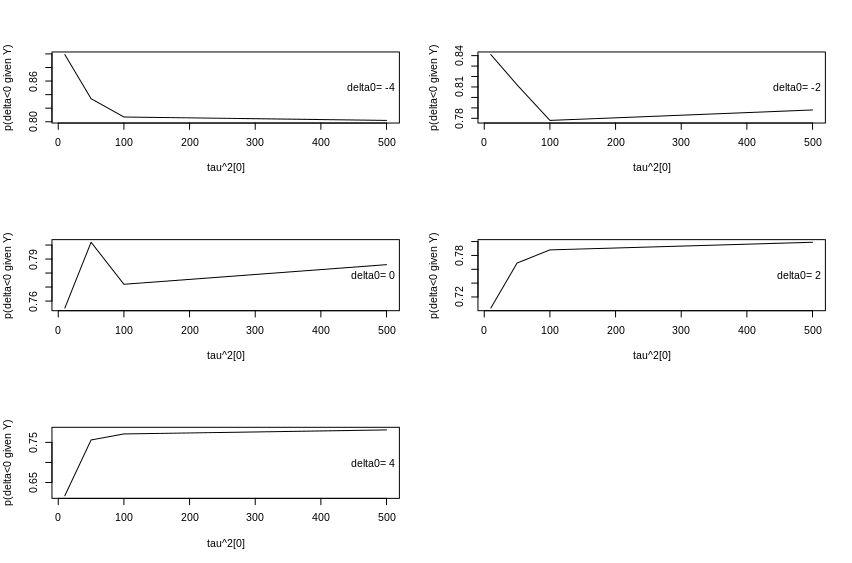
\includegraphics[scale = 0.7]{img/esercizio8-2-1}
 \caption{probabilità a posteriori al variare della prior}
 \label{figure:figura12}
\end{figure}

\begin{lstlisting}[style=R]

#a)ii
\end{lstlisting}
{
\color{red}
\begin{Verbatim}
> quantili.post
                        2.5%    97.5%
delta0=-4 tau20=10  -4.166501 0.885176
delta0=-4 tau20=50 -4.080470 1.261487
delta0=-4 tau20=100 -3.966220 1.815875
delta0=-4 tau20=500 -3.984476 1.560537
delta0=-2 tau20=10  -3.921579 1.224411
delta0=-2 tau20=50  -3.987036 1.520727
delta0=-2 tau20=100 -3.956075 1.720433
delta0=-2 tau20=500 -3.794180 1.702581
delta0=0 tau20=10   -3.459266 1.618012
delta0=0 tau20=50   -3.884302 1.613191
delta 0=0 tau20=100 -4.000856 1.521053
delta0=0 tau20=500  -4.081757 1.850854
delta0=2 tau20=10   -3.017789 1.890537
delta0=2 tau20=50   -3.727812 1.800686
delta0=2 tau20=100  -3.664780 1.952699
delta0=2 tau20=500  -4.089526 1.830220
delta0=4 tau20=10   -2.637665 2.135446
delta0=4 tau20=50   -3.850333 1.857685
delta0=4 tau20=100  -3.661231 1.695296
delta0=4 tau20=500  -4.298413 1.823357
\end{Verbatim}
}


\begin{lstlisting}[style=R]
#Per quanto riguarda gli intervalli di credibilita' per delta si osserva
#quanto appena notato per la precedente #probabilita': la distribuzione a
#priori influisce piu' dei dati sull'inferenza a posteriori quanto piu' e'
#informativa.

#a)iii

#Confrontiamo ora le correlazioni a priori e quelle #a posteriori fra le
#medie dei due gruppi thetaA=mu+delta e thetaB=mu-delta.
#La correlazione a priori si puo' calcolare #analiticamente e rimandiamo per
#questo a i passaggi precedenti al codice e riportiamo di seguito i valori
#per ogni combinazione degli iperparametri della prior su delta):

correlazione.prior<-c(0.81,0.33,0,-0.67)

#Le correlazioni a posteriori precedentemente calcolate invece sono:
}

\end{lstlisting}

{
\color{red}
\begin{Verbatim}
> correlazione.post
              tau20=10    tau20=50    tau20=100    tau20=500
  delta0=-4 0.11470736  0.04394125 -0.014843283 -0.047380931
  delta0=-2 0.05693164  0.04900340 -0.081550575 -0.007036669
  delta0=0  0.06714184  0.03791250 -0.008966994 -0.026858228
  delta0=2  0.11899453  0.04389222 -0.009447653 -0.044961021
  delta0=4  0.13144920 -0.03688193  0.005192835 -0.064853163
\end{Verbatim}
}


\begin{lstlisting}[style=R]
#Si osserva che le correlazioni a posteriori tra le medie dei due gruppi
#sono pressoche' nulle per tutte le possibili specificazioni della prior
#su delta; a priori invece si osserva che la correlazione e' molto alta in
#direzione positiva per specificazioni di prior molto informative e
#viceversa decresce fino a valori negativi per prior sempre piu' diffuse.


#b)

#Il confronto tra le due medie di gruppo thetaA e thetaB puo' essere
#ricondotto al parametro delta, semi-differenza tra le due medie,
#per come e' stato formulato il modello gerarchico: in questo caso thetaA
#e' minore di thetaB se delta e' minore di z e ro. Possiamo pertanto usare i
#risultati del punto precedente per descrivere come cambia l'evidenza che
#thetaA sia minore di thetaB tra persone che hanno opinioni molto diverse
#tra loro.
#Per quanto prima osservato risulta che l'inferenza a posteriori segue
#la direzione che ci aspettiamo in base alla distribuzione a priori
#specificata: le prior della semi differenza piu' informative e centrate su
#valori negativi hanno un peso maggiore dei dati e viceversa. Vediamolo di
#seguito riportando alcuni plot che mettono a confronto la distribuzione a
#priori e quella a posteriori di delta, in particolare quelli per delta0=-4
#in cui varia tau2 e quelli per delta0=4 in cui varia tau2 (situazioni
#estreme)

win.graph()
par(mfrow=c(2,2))
x<-seq(-50,50,by=0.01)
v<-0
for(j in 1:4){
  plot(x,dnorm(x,delta0[1],sqrt(tau20[j])), xlim=c(-10,10),ylim=c(0,0.3),
  xlab=expression(delta),ylab="density",type="l",col="grey")
  lines(density(gibbs[,2,j]))
  legend("topright",legend=c("posterior","prior"),lwd=c(2,2),col=c("black",
  "gray"),bty="n")
  text(5.5,0.15,paste("tau20=",tau20[j]))
}

win.graph()
par(mfrow=c(2,2))
x<-seq(-50,50,by=0.01)
v<-0
for(j in 1:4){
  plot(x,dnorm(x,delta0[5],sqrt(tau20[j])),xlim=c(-10 ,10),ylim=c(0,0.3),
  xlab=expression(delta),ylab="density",type="l",col="grey")
  lines(density(gibbs[,2,j+16]))
  legend("topright",legend=c("posterior","prior"),lwd=c(2,2),col=c("black",
  "gray"),bty="n")
  text(5.5,0.15, paste("tau20=",tau20[j]))
}

\end{lstlisting}
\begin{figure}
 \centering
 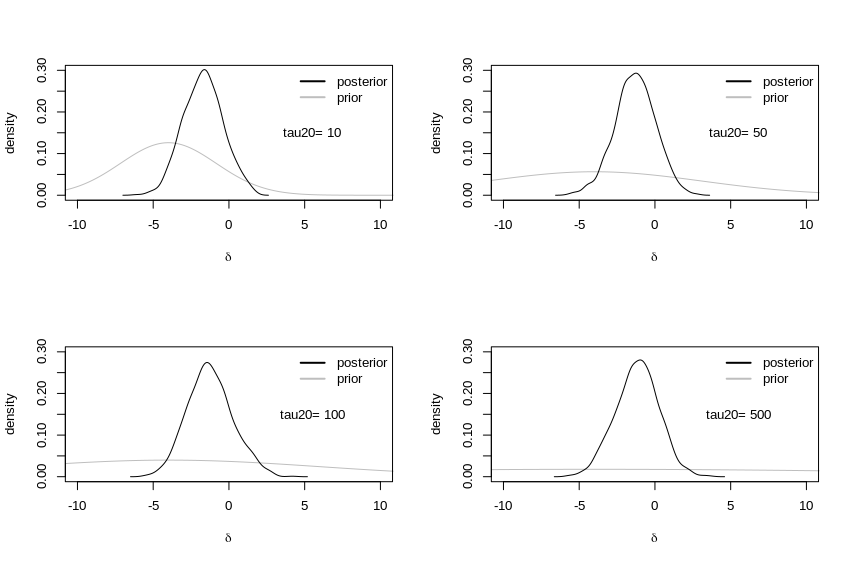
\includegraphics[scale=0.7]{img/esercizio8-2-2}
 \caption{densita' a posteriori al variare della prior}
 \label{figure:figura13}
\end{figure}

\begin{figure}
 \centering
 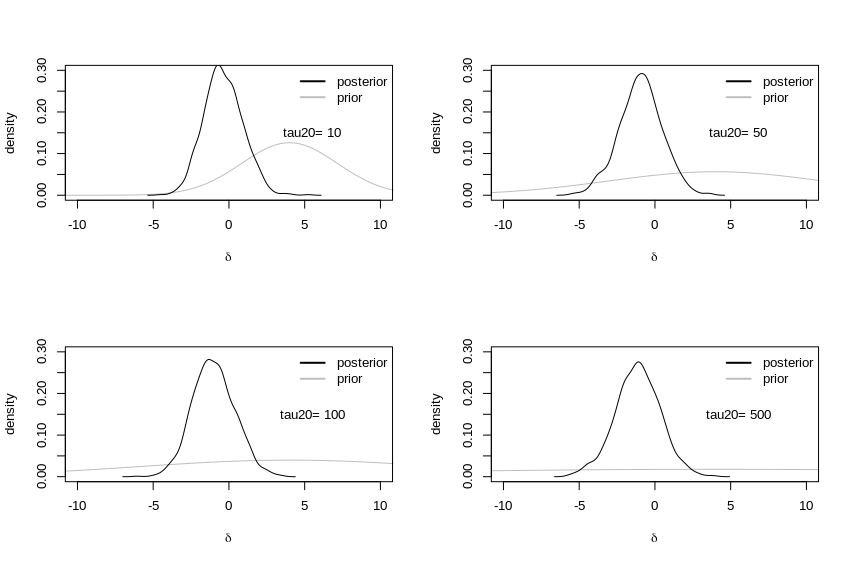
\includegraphics[scale=0.7]{img/esercizio8-2-3}
 \caption{densita' a posteriori al variare della prior}
 \label{figure:figura14}
\end{figure}
\begin{lstlisting}[style=R]

#Come sempre facciamo una veloce verifica della convergenza dell'algoritmo:
#library(coda)
effectiveSize(gibbs[,,1])
\end{lstlisting}

{
\color{red}
\begin{Verbatim}
  mu  delta  sigma2
1000   1000    1000
\end{Verbatim}
}



\end{itemize}

